\documentclass[11pt,a4paper]{article}
\usepackage[margin=24mm]{geometry}
\usepackage[T1]{fontenc}
\usepackage{lmodern,amsmath,amssymb,mathtools,graphicx,booktabs,array}
\usepackage[colorlinks=true,linkcolor=blue!50!black,urlcolor=blue!60!black,citecolor=blue!50!black]{hyperref}
\usepackage{xcolor}
\usepackage{microtype}
\usepackage{float,placeins}
\usepackage{fancyhdr}
\pagestyle{fancy}\fancyhf{}\fancyhead[L]{\small Dalitz integrals and analytic continuation}\fancyhead[R]{\small Research note}\fancyfoot[C]{\thepage}
\setlength{\headheight}{14pt}
\newcommand{\dd}{\,\mathrm d}
\newcommand{\Disc}{\operatorname{Disc}}
\newcommand{\phys}{\mathrm{phys}}
\newcommand{\INT}{\mathrm{INT}}
\newcommand{\QTB}{\mathrm{QTB}}
\title{Resolving the Appendix C continuation problem\\[3pt]\large Physical boundary values, lifted contours, and a constructive local solution}
\author{Research scratchpad for \texttt{PolePositionOfA1fromTau}}
\date{15 October 2026}
\begin{document}
\maketitle
\begin{abstract}
Appendix C of Ref.~\cite{paper} exposes a genuine tension: preserving the physical Dalitz integral seems to require a special contour through a threshold-touching point, whereas ordinary contour continuation suggests avoiding that point and following one analytic branch. We first reconstruct why the second choice is natural, using the original endpoint and contour plots. We then distinguish analyticity in the integration variable from analyticity of the completed integral in total energy. Reversing the integration order solves the toy problem independently; a two-sector construction preserves the physical boundary values, while an explicit correction relates it to the alternative lift. Numerical checks and the full rho model clarify both the resolution and its limits. Global contour transport to the resonance pole remains a separate task.
\end{abstract}


\section{Why the second choice is natural}
Before resolving the issue, we should recover the reason it was an issue. The two choices prioritize two legitimate requirements: reproducing the physical Dalitz domain, and keeping the inner integral analytic as the outer contour is deformed. Choice 2 follows the usual instincts of complex contour integration. Its appeal is not an arbitrary preference for a different square-root sign.

For this discussion write $u=\sigma_1$, $v=\sigma_3$, $a=4m_\pi^2$, $b(s)=(\sqrt{s}-m_\pi)^2$, and $u_0(s)=(s-m_\pi^2)/2$. At fixed $s$, the outer variable runs from $a$ to $b$ and the inner contour connects $v_-(u;s)$ to $v_+(u;s)$. The toy kernel is $1/\sqrt{v-a}$. We will distinguish the projected endpoint $v_-$ from its location on the two-sheeted square-root surface.

\subsection{First follow the moving endpoint}
Figure~\ref{fig:original-endpoints} is the original Fig.~13, extracted from the paper. Read it from left to right, following increasing outer-contour parameter $x$, where $u=a+x(b-a)$.

\begin{figure}[H]\centering
\includegraphics[page=18,trim=33 535 33 45,clip,width=.96\textwidth]{sources/1810.00016.pdf}
\caption{Original Fig.~13 of Ref.~\cite{paper}, reproduced from arXiv v2, p.~18. Left: real parts of the two moving endpoints. Right: imaginary parts for a small positive imaginary part of $s$. The insets resolve the lower endpoint's passage around the threshold. The vertical red marker indicates the outer path's closest approach to $u_0$; it does not mean that the path passes exactly through $u_0$.}
\label{fig:original-endpoints}
\end{figure}

\paragraph{Read the left panel first.} The lower endpoint approaches the horizontal threshold level $a$, turns, and returns. In the strictly real physical Dalitz plot it touches threshold at $u=u_0$. At the outer endpoint $u=b$, the upper and lower inner endpoints meet, so the physical inner interval closes. Seen only through real parts, nothing seems to demand a change of sheet.

\paragraph{Then inspect the right panel and both insets.} Once $s$ has a small imaginary part and $u$ follows the straight path, $v_-$ no longer merely touches $a$. Its imaginary part changes sign while its real part passes to the left of threshold: the endpoint goes around the branch point. The excursion can be extremely small in the projected plane, but it is not small topologically for a square root. Following the root continuously changes its sheet.

This is the motivation for choice 2: transport the inner contour with its endpoints, avoid its singularities, and follow the square root continuously. Do not reset its sign after the excursion. When the projected endpoints eventually coincide at $u=b$, their lifted endpoints can still occupy different sheets. The transported inner contour then need not shrink to zero.

\subsection{Now look from the outer-contour perspective}
After performing the inner integral, the toy integrand contains $\sqrt{v_-(u;s)-a}$. Figure~\ref{fig:original-contour}, the original Fig.~14, displays the resulting cut prescription in the complex $u$ plane.

\begin{figure}[H]\centering
\includegraphics[page=19,trim=155 575 110 35,clip,width=.61\textwidth]{sources/1810.00016.pdf}
\caption{Original Fig.~14 of Ref.~\cite{paper}, reproduced from arXiv v2, p.~19. The green dashed outer contour goes through a generic waypoint $P$. The special marked point is $u_0=(s-m_\pi^2)/2$. Red curves depict the cuts in the paper's chosen representation; the local status of the double zero at $u_0$ will be examined below.}
\label{fig:original-contour}
\end{figure}

\paragraph{Start with the green path.} A generic waypoint $P$ is attractive: contours should be deformable as long as singularities are avoided and the sheet is followed consistently. In the full calculation this freedom is useful for taking the hook contour around the rho pole. Choice 2 preserves a single analytic inner-integral branch along that deformed outer path.

\paragraph{Now move $P$ exactly onto the marked point $u_0$.} This is the special route of choice 1. The lower inner endpoint touches its threshold instead of going around it, and the physical prescription can remain on the same $v$ sheet on either side of the touch. But the inner integral is then not represented by one analytic branch across $u_0$ as a function of $u$. Why should a path passing \emph{exactly} through the special point be privileged over an arbitrarily close detour? From the perspective of standard contour deformation, choice 1 looks exceptional, and choice 2 looks more natural.

The question is therefore substantial: \emph{does preserving the physical integral force us to sacrifice the analyticity needed to deform contours?} The paper's two choices expose this tension rather than merely an incorrect square-root evaluation.

\subsection{A local picture of the competing requirements}
Figure~\ref{fig:root-lift} isolates the issue on the real physical interval. Its solid curve is the positive endpoint root $q_-^{\phys}=\sqrt{v_--a}$. The dashed curve, denoted by $h$, agrees with it before the touching point and is then followed as one analytic function of $u$. The exact formula for $h$ will be derived below.

\begin{figure}[H]\centering
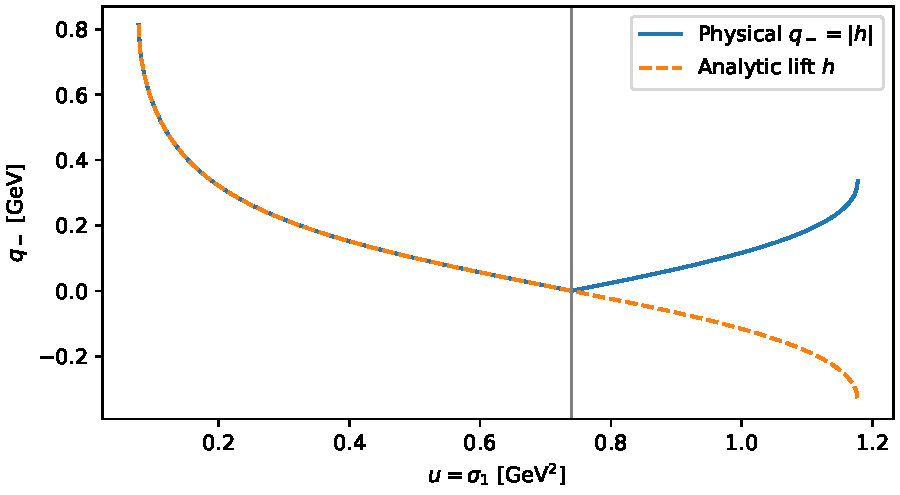
\includegraphics[width=.76\textwidth]{figures/root_lift.pdf}
\caption{Two requirements seen in one real-axis plot, at $s=1.5\ \mathrm{GeV}^2$. Solid: the positive lower-endpoint root required by the physical Dalitz integral. Dashed: one analytic lift in the outer variable. They coincide to the left of the vertical line $u=u_0$ and differ to its right. This figure explains the appeal of choice 2 before deciding which completed integral is required.}
\label{fig:root-lift}
\end{figure}

\paragraph{To the left of the vertical line, there is no choice to make.} Both curves describe the same root. At the line, that root vanishes. To the right, the solid curve turns upward to remain the physical positive root; the dashed curve passes smoothly through zero and becomes negative. Locally the distinction is the one between $|u-u_0|$ and a signed analytic multiple of $u-u_0$.

The dashed curve is natural if the question is ``which branch is analytic in the integration variable $u$?'' The solid curve is required if the question is ``which lower endpoint reproduces the physical Dalitz integral?'' Calling the dashed curve simply wrong would miss the reason for introducing it.

\paragraph{The question that opens the way forward.} We ultimately need the \emph{completed integral} to be analytic in total energy $s$. Must its inner integral also be represented by one analytic branch across the whole outer contour in $u$? The answer will be no: two separately continued sectors can preserve the physical domain and yield an analytic function of $s$. The next sections establish that statement independently and then show how to retain contour-deformation freedom with the appropriate correction.
\FloatBarrier

\section{What are we trying to continue?}
The immediate objective is to continue the \emph{specified real-axis spectral function} $\rho(s)$ into a complex neighbourhood of an open interval $s>9m_\pi^2$, and then transport that analytic germ along a specified path to the resonance sheet. It is not necessary for every nested-integral representation to have an integrand analytic in its outer integration variable across the entire physical contour.

Three objects must be distinguished:
\begin{enumerate}
\item The phase-space spectral density, obtained from the physical Dalitz integral. Its off-axis extension is a local analytic germ; the Heaviside prescription setting it to zero below threshold is not continued as a holomorphic function.
\item The first-sheet dispersive loop, fixed by that real spectral density, a subtraction prescription, and any stated additional analytic terms.
\item The adjacent-sheet loop, obtained by continuing through the physical cut. Its value additionally depends on the continuation path around further singularities.
\end{enumerate}
To fix signs explicitly, define a loop with $\Disc L=2i\rho$:
\begin{equation}
 L^{\mathrm I}(s)=L(s_*)+\frac{s-s_*}{\pi}
 \int_{9m^2}^{\infty}\frac{\rho(x)\dd x}{(x-s_*)(x-s)},\qquad s_*<9m^2.
 \label{eq:disp}
\end{equation}
On the lower-half-plane chart reached from the upper rim,
\begin{equation}
 L^{\mathrm {II}}(s)=L^{\mathrm I}(s)+2i\rho_{\phys}(s).
 \label{eq:second}
\end{equation}
Indeed $L^{\mathrm I}(x-i0)+2i\rho(x)=L^{\mathrm I}(x+i0)$. The inverse amplitude in the repository uses $L=i\widetilde\rho$ and $t^{-1}=K^{-1}-L/2$; hence its lower-half-plane formula has the additional term $-i\rho_{\phys}$. Signs must be tied to the rim and chart, not to a bare ``sheet II'' label.

\paragraph{A decisive question.} Do the two proposed continuations recover exactly the same function on an open physical interval? If not, they are not competing continuations of that function. If both are holomorphic in a common neighbourhood and agree there on the real interval, the identity theorem forces equality. Global monodromy remains possible when their continuation paths wind differently around actual singularities.

\paragraph{What the paper already establishes.} Section IV B explicitly states that its second prescription changes the physical-axis interference and gives a correction integral, Eq.~(28). The paper also already recognizes cancellation of the explicit breakup-momentum factor in the full integrand. Those observations are correct and are essential to the diagnosis below. The new step here is an explicit construction showing that the physical choice is analytically continuable despite its piecewise outer-integrand representation.

\section{An exact reduction of the Appendix C toy problem}
Write $m=m_\pi$, $M=m^2$, and introduce
\begin{equation}
 a=4M,\quad b=(\sqrt{s}-m)^2,\quad c=(\sqrt{s}+m)^2,
 \quad u_0=\frac{s-M}{2}.
\end{equation}
For $s>9M$, $a<u_0<b$. Set $u=\sigma_1$, $v=\sigma_3$. The Dalitz endpoints are
\begin{equation}
 v_\pm(u;s)=\frac{s+3M-u}{2}
 \pm\frac{\sqrt{u-a}\sqrt{(b-u)(c-u)}}{2\sqrt u},
 \label{eq:endpoints}
\end{equation}
with positive roots on the physical interval. Appendix C considers
\begin{equation}
 X_{\phys}(s)=\int_a^b\dd u\int_{v_-}^{v_+}\frac{\dd v}{\sqrt{v-a}}.
 \label{eq:toy}
\end{equation}

\subsection{Reverse the order before continuing}
On the real physical Dalitz plot, interchange of the two equal-mass pair invariants leaves the domain unchanged. The integrand is integrable, so reversing the order is legitimate. The width of the allowed $u$ interval at fixed $v$ is
\begin{equation}
 u_+(v;s)-u_-(v;s)=\frac{\sqrt{v-a}\sqrt{(b-v)(c-v)}}{\sqrt v}.
\end{equation}
The threshold factor cancels, giving the exact identity
\begin{equation}
 \boxed{X_{\phys}(s)=\int_a^b\frac{\sqrt{b-v}\sqrt{c-v}}{\sqrt v}\dd v.}
 \label{eq:reverse}
\end{equation}
With $v=a+(b-a)t$, it becomes
\begin{equation}
 X_{\phys}(s)=(b-a)^{3/2}\int_0^1
 \frac{\sqrt{1-t}\sqrt{c-a-(b-a)t}}{\sqrt{a+(b-a)t}}\dd t.
 \label{eq:fixed}
\end{equation}
Continue every root from a fixed physical reference point. Around any such point above threshold, the fixed-interval integral is holomorphic in $s$: the denominator stays nonzero and the endpoint factor is uniformly integrable. This proves existence and selects the physical germ without first resolving the special outer-contour prescription.'' Further away, roots and contours still need tracking.

\subsection{What happens at \texorpdfstring{$u_0$}{u0}?}
Direct algebra gives
\begin{equation}
 (v_+-a)(v_--a)=\frac{M}{u}(s-M-2u)^2
 =\frac{4M}{u}(u-u_0)^2.
 \label{eq:identity}
\end{equation}
Define, locally near the physical contour,
\begin{equation}
 q_+=\sqrt{v_+-a},\qquad
 h(u,s)=\frac{2m(u_0-u)}{\sqrt u\,q_+}.
 \label{eq:h}
\end{equation}
Then $h^2=v_--a$, and $h$ is an analytic lift near $u_0$, with a simple zero there. The physical root is instead
\begin{equation}
 q_-^{\phys}=\sqrt{v_--a}=
 \begin{cases}h,&a\leq u\leq u_0,\\-h,&u_0\leq u\leq b.\end{cases}
 \label{eq:physicalroot}
\end{equation}
It has an absolute-value cusp as a function of real $u$.

A double zero inside a square root is not a ramification point of its locally normalized algebraic surface. Locally $\sqrt{(u-u_0)^2A(u,s)}=\pm(u-u_0)\sqrt{A(u,s)}$ when $A\ne0$. Thus ``two adjoined square-root branch points'' is a potentially misleading description: a principal-value implementation has a seam, while the two analytic lifts are locally regular. The physical prescription changes between those lifts. In Eq.~(C3), the endpoint that actually reaches $a$ on the physical branch is $v_-$; writing $v_+$ after squaring loses the endpoint/branch information.

Return now to Fig.~\ref{fig:root-lift}: Eq.~\eqref{eq:h} is the dashed curve, while Eq.~\eqref{eq:physicalroot} is the solid curve. The local identity explains precisely why the dashed curve crosses zero and the solid curve turns back. The distinction anticipated in the figure is therefore algebraic, not a numerical branch-selection accident.

\subsection{A constructive physical continuation}
Since the primitive in $v$ is $2\sqrt{v-a}$, the physical answer is
\begin{equation}
 \boxed{X_{\phys}(s)=2\int_a^{u_0}(q_+-h)\dd u
                 +2\int_{u_0}^{b}(q_++h)\dd u.}
 \label{eq:split}
\end{equation}
Map each outer segment separately to $[0,1]$ and continue its endpoints and its branch assignments in $s$. Each term then has a locally holomorphic, fixed-parameter representation. Their sum is holomorphic in $s$, even though the unsplit integrand is not analytic across $u_0$ in $u$.

The special point is a \emph{moving sector boundary}, not an obstruction to analyticity of the integrated function. Each sector contour can be deformed independently on its own sheet as long as singularities are avoided. There is no requirement that a single analytic lift in $u$ represent both sectors.

\subsection{The other function and the missing piece}
Let $X_{\mathrm{lift}}$ be the prescription that follows $h$ analytically all the way from $a$ to $b$:
\begin{equation}
 X_{\mathrm{lift}}(s)=2\int_a^b(q_+-h)\dd u.
\end{equation}
It is the toy realization of the alternative lift discussed in Appendix C. On the physical axis,
\begin{equation}
 \boxed{X_{\mathrm{lift}}-X_{\phys}
 =-4\int_{u_0}^b h\dd u
 =4\int_{u_0}^b\sqrt{v_--a}\dd u>0.}
 \label{eq:correction}
\end{equation}
The first expression on the right also gives the locally continued correction. The second expression is a real-axis formula with the positive root. The sign is fixed by our choice that $h>0$ on the first sector; reversing conventions changes how the correction is written, not the physical answer.

At $u=b$, the projected endpoints $v_+$ and $v_-$ coincide. The physical fiber shrinks to zero. The single-lift prescription instead has $q_-=-q_+$ there, so its fiber runs between different points above the same projected $v$. It is a nontrivial cycle on the square-root surface. Projection to the complex $v$ plane conceals that difference.

One can consequently use a convenient alternative contour \emph{provided the transported correction chain is also included}. Equation~\eqref{eq:correction} is an explicit example of that rule. Analyticity of an integrand along a chosen contour is insufficient to establish that the contour represents the desired physical integral.

\section{Limiting cases that select the answer}
\subsection{Three-pion threshold}
Let $\delta=b-a\to0^+$. From Eq.~\eqref{eq:fixed}, $c\to16M$, giving
\begin{equation}
 X_{\phys}(s)=\frac{2\sqrt3}{3}\delta^{3/2}[1+O(\delta/M)],
 \qquad \delta=\frac23(s-9M)+O((s-9M)^2/M).
 \label{eq:threshold}
\end{equation}
The physical noninteger power is a genuine threshold singularity in $s$; it is unrelated to the interior cusp at $u_0$. A calculation yielding a different coefficient or threshold power fails a strong boundary check.

\subsection{Massless limit}
At $m=0$, the Dalitz domain is the triangle $0<u<s$, $0<v<s-u$. Direct evaluation gives
\begin{equation}
 X(s)=\int_0^s\dd u\int_0^{s-u}\frac{\dd v}{\sqrt v}
      =\frac43s^{3/2}.
\end{equation}
The correction in Eq.~\eqref{eq:correction} disappears in this limit. Thus agreement in the massless limit alone cannot distinguish the two finite-mass prescriptions. This is a useful example of a limit that checks a calculation without resolving every ambiguity.

\subsection{Remove the subchannel cut}
If the full reduced kernel is analytic and single-valued in $v$ near $a$, then $v=a+q^2$ gives a differential $2qG(a+q^2)\dd q$ with an even primitive. Changing the sign of the lower $q$ endpoint changes nothing. The two prescriptions coincide in this controlled case. They differ only through the part of the full kernel that is sensitive to the subchannel sheet.

\subsection{Stable-isobar limit}
For a normalized narrowing isobar spectral distribution,
\begin{equation}
 \frac{\sqrt{1-4M/\sigma}|f_\rho(\sigma)|^2}{16\pi^2}
 \longrightarrow\delta(\sigma-m_\rho^2),
\end{equation}
so the QTB integral becomes
\begin{equation}
 \rho_\QTB(s)\longrightarrow
 \frac{\sqrt{\lambda(s,m_\rho^2,M)}}{8\pi s}
\end{equation}
above its threshold. Its nearby complex threshold tends to $(m_\rho+m)^2$. The stable two-body continuation fixes the sheet choice here. This normalized distributional limit is different from merely setting the running width to zero with a fixed numerator; the latter can generate real-axis poles and is only safe away from them.

\section{Numerical checks of the toy solution}
The script \texttt{continuation\_checks.py} uses Gauss--Legendre integration with a $\sin^2$ endpoint map. The two-sector formula uses 180 nodes per segment; the reversed integral uses 240. It checks their equality, Eq.~\eqref{eq:correction}, and invariance under a small complex bend of each sector contour. The algebraic identity~\eqref{eq:identity} is also checked symbolically.

\begin{table}[ht]\centering\small
\begin{tabular}{@{}lll@{}}\toprule
$s$ [$\mathrm{GeV}^2$] & $X_{\phys}$ [$\mathrm{GeV}^3$] & $X_{\mathrm{lift}}-X_{\phys}$ [$\mathrm{GeV}^3$]\\\midrule
$0.2$ & $0.002529394948$ & $0.000395254123$\\
$0.5$ & $0.150273862202$ & $0.022841567816$\\
$1.5$ & $1.492210355046$ & $0.188433937364$\\
$1.5-0.05i$ & $1.491168982777-0.091321734489i$ & $0.188368579957-0.010129758482i$\\
$1.5-0.6i$ & $1.343770765060-1.105827987706i$ & $0.179305878400-0.122923282787i$\\\bottomrule
\end{tabular}
\caption{Independent physical representations agree within $4\times10^{-15}$ relatively at these points. These digits describe numerical agreement, not an error bound for an unspecified global continuation.}
\end{table}

For $s-9M=10^{-3},10^{-4},10^{-5}\ \mathrm{GeV}^2$, the computed ratio $X/\delta^{3/2}$ is $1.1553563$, $1.1547664$, $1.1547071$, tending to $2\sqrt3/3=1.1547005$. At $m=0$ and $s=1.5\ \mathrm{GeV}^2$, the result is $2.449489742783$, as predicted.

\begin{figure}[H]\centering
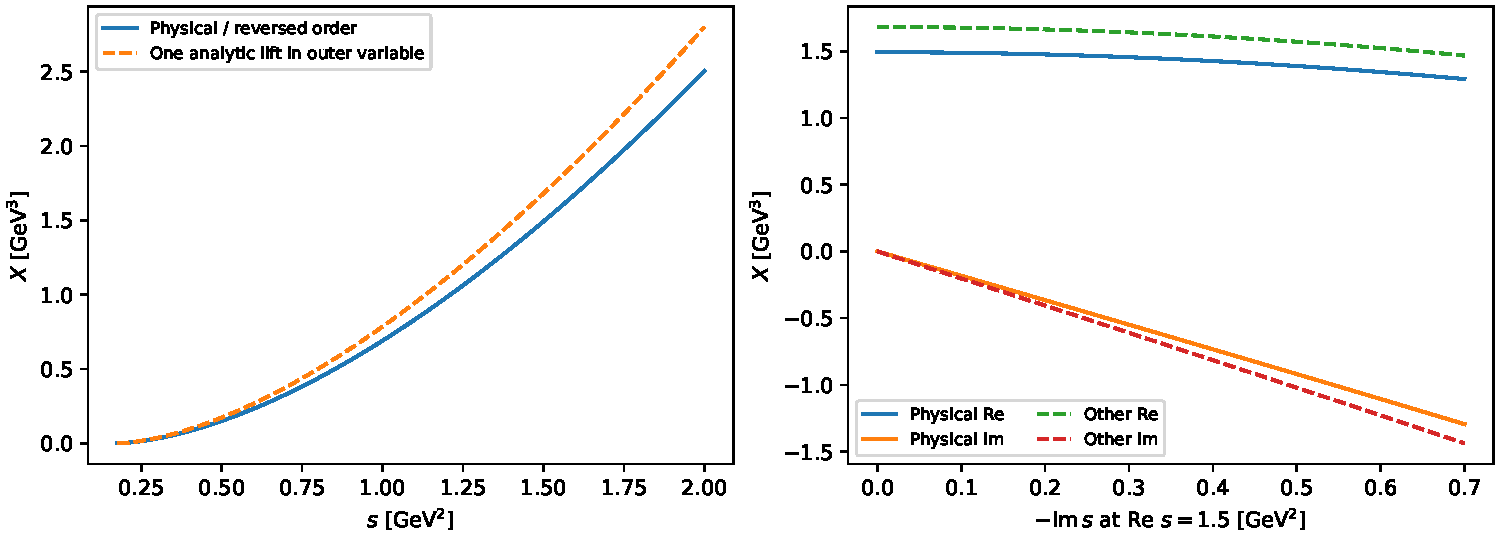
\includegraphics[width=\textwidth]{figures/toy_continuation.pdf}
\caption{Integrated consequences of the branch distinction in Fig.~\ref{fig:root-lift}. Left: physical and single-lift toy functions on the real axis. Right: their real and imaginary parts along $s=1.5-i y\ \mathrm{GeV}^2$. Solid lines preserve the physical Dalitz integral; dashed lines follow the alternative lift.}
\label{fig:toy-values}
\end{figure}

\paragraph{Read Fig.~\ref{fig:toy-values} back against the endpoint plot.} In the left panel, the dashed function lies above the solid one because the negative part of $h$ in Fig.~\ref{fig:root-lift} is subtracted in the inner primitive. Equation~\eqref{eq:correction} makes that extra contribution positive. The separation already on the real axis tells us that the two constructions start from different integrated data; it is not evidence that a single analytic germ has two values.

In the right panel, start at $y=0$. The real parts are already separated, while both imaginary parts vanish. As $y$ increases, both functions develop smooth complex values, and their separation persists. Smoothness of both curves is entirely consistent with the author's observation that both choices give analytic functions. The physical boundary condition, together with the continuation path, is what selects the desired one.
\FloatBarrier

\section{The full interference: cancellation helps, but does not remove the issue}
The physical integrand in Eq.~(B16) can be written as
\begin{equation}
 \rho_\INT(s)=\frac{1}{2\pi(8\pi)^2s}\int\dd u\int\dd v\,
 R_-(u)R_+(v)\mathcal K(s,u,v),
 \label{eq:full}
\end{equation}
where $R_+=f_\rho/\sqrt{\sigma-a}$, $R_-$ continues its real-axis conjugate, and
\begin{equation}
 \mathcal K(s,u,v)=\frac{W(\sqrt s,\sqrt u,\sqrt v)}
 {[(\sqrt s+\sqrt u)^2-M][(\sqrt s+\sqrt v)^2-M]}.
\end{equation}
Here $W$ is the polynomial given in the paper. Our $\rho_\INT$ follows the paper's convention $\rho_{\mathrm{SYMM}}=\rho_\QTB-\rho_\INT$. The code's \texttt{interference} includes the opposite sign through \texttt{angular\_pow2}, and adds that quantity to QTB.

Conjugation must be continued as a separate analytic factor: on an appropriate local chart $f^\sharp(z)=\overline{f(\bar z)}$. Replacing it by $\overline{f(z)}$ at complex $z$ would not be holomorphic. The repository's paired \texttt{f1\_I}/\texttt{f1\_II} functions serve this purpose locally; their names alone do not specify every global branch convention.

\subsection{Why the toy mismatch is much larger}
For the running-width $P$-wave rho model, write $\sigma=a+q^2$. After canceling the numerator threshold factor,
\begin{equation}
 R_\pm(a+q^2)=\frac{A(q^2)}{D(q^2)\mp iB(q^2)q^3},
 \label{eq:reduced}
\end{equation}
where $A,B,D$ are analytic near $q=0$, and $D(0)\ne0$. The Blatt--Weisskopf and $\sqrt\sigma$ factors are included in these functions; their more distant singularities remain relevant globally.

Near threshold the sheet-sensitive part starts at $q^3$, not $1/q$. Multiplication by $\dd v=2q\dd q$ makes its primitive start at $q^5$. Thus the difference of endpoint lifts is suppressed by at least five powers of the small endpoint momentum in the inner primitive. The angular kernel can suppress it further; it actually vanishes at $u=u_0,v=a$. This is a mechanism for small differences, not a uniform numerical bound near resonance poles.

The toy integrand $1/q$ gives $2\dd q$ and a primitive linear in $q$, so it exaggerates the endpoint sensitivity. The physical cancellation does \emph{not} make the full amplitude single-valued: the $q^3$ running width retains a true subchannel branch dependence.

\subsection{A practical local prescription}
The following construction removes the ambiguity without requiring numerical integration through a divergent endpoint:
\begin{enumerate}
\item Split $u$ into $a\to u_0(s)$ and $u_0(s)\to b(s)$.
\item On each sector choose $q_-=h$ or $-h$, respectively, and the same transported $q_+$ as above.
\item Parameterize the inner path on the uniformized surface,
\begin{equation}
 q=q_-+y(q_+-q_-),\quad v=a+q^2,\quad
 \dd v=2q(q_+-q_-)\dd y,\qquad 0\leq y\leq1.
\end{equation}
\item Evaluate the reduced isobar factors directly as functions of $q$, not by recomputing a principal $\sqrt{v-a}$ after projecting back to $v$.
\item Continue the two fixed-parameter integrals from a physical reference point. Deform paths when an isobar pole or another singularity approaches; retain the sheet and chain information.
\end{enumerate}
At $q=0$ the complete integrand is regular. At physical $s$ this is exactly a change of variables in the original Dalitz integral. Local holomorphy then establishes that it is the desired germ. A convenient global path can include hooks, but those must be transported from these initial chains or accompanied by their correction terms.

\subsection{Checks with the full rho model}
The prototype uses the masses, width and $R=5\ \mathrm{GeV}^{-1}$ from \texttt{src/Isobars.jl}, and the factorized angular polynomial. The common normalization factor \texttt{ns1} is omitted in all entries below; it cancels in every relative comparison. The single-lift column uses $q_-=h$ on both sectors. It illustrates the same change of integration chain; it is not a bit-for-bit reproduction of the repository's hook contour.

\begin{table}[ht]\centering\small
\begin{tabular}{@{}lll@{}}\toprule
$s$ [$\mathrm{GeV}^2$] & Physical interference, unnormalized & Relative lift mismatch\\\midrule
$0.5$ & $-3.16414762935\times10^{-5}$ & $2.1593\times10^{-4}$\\
$1.5$ & $-2.65407186784\times10^{-4}$ & $3.9366\times10^{-4}$\\
$1.5-0.02i$ & $-2.65402990618\times10^{-4}-2.96346220626\times10^{-6}i$ & $3.9089\times10^{-4}$\\\bottomrule
\end{tabular}
\caption{Relative mismatch is $|\rho_{\mathrm{lift}}-\rho_{\phys}|/|\rho_{\phys}|$ for the interference alone, not for the total spectral density.}
\end{table}

Independent real-axis integration in $(u,v)$ agrees with the physical $(u,q)$ calculation. Increasing the sector quadrature from 180 to 260 nodes changes these values by less than $4\times10^{-14}$ relatively. Exchanging the two conjugate isobar assignments, equivalent to interchanging $u$ and $v$ in the physical integral, agrees within $6\times10^{-14}$. A finite-difference Cauchy--Riemann check at $s=1.5-0.02i$ gives a relative residual $1.7\times10^{-10}$ for a step $10^{-5}\ \mathrm{GeV}^2$.

As a further controlled test, scale only the running width by $\eta$ and take $s=0.3\ \mathrm{GeV}^2$, safely below the rho pole in the subchannel integration range. For $\eta=1,0.1,0.01,0$, the absolute lift differences are approximately $2.02\times10^{-10}$, $2.03\times10^{-11}$, $2.03\times10^{-12}$, and $2.1\times10^{-21}$ in the common unnormalized convention. This isolates the sheet-dependent running width and confirms that the mismatch vanishes when the relevant subchannel cut is removed.

\section{What remains serious: transport to the pole}
The interior touching point $u_0$ is not itself a new singularity in total energy. Genuine obstructions arise when singularities pinch the continued integration chain, or collide with its endpoints so that no local deformation preserves it. The familiar isobar--spectator branch point is obtained when
\begin{equation}
 b(s)=\sigma_\rho^{\mathrm{pole}},\qquad
 s_{\rho\pi}=(m+\sqrt{\sigma_\rho^{\mathrm{pole}}})^2.
\end{equation}
Crossed-channel singularities, additional poles of the parametrization, and left-hand cuts also require inspection. A contour crossing at a particular numerical representation is not automatically a singularity of the integral: first try deforming the contour. A pinch that cannot be removed is a different matter.

\paragraph{A deliberately failed global check.}
For the undeformed sector paths, the full-model scan at $s=1.5-0.1i$ passes refinement and exchange checks. At $s=1.5-0.3i$, the 180-to-260-node relative change is about $1.07$, and the exchange discrepancy is about $3.80$. This is an unmistakable failure of that quadrature/contour chart, and a direct pole-location check confirms the crossing. The inner reduced isobar has a pole at $q_\rho=0.72245985-0.08053124i\ \mathrm{GeV}$, or $v_\rho=0.59338209-0.11636118i\ \mathrm{GeV}^2$. With a linear outer sector coordinate $u=\ell+(r-\ell)t$, this pole lies on the inner integration path at $(t,y)=(0.927396,0.848555)$ in the first sector and $(0.024321,0.888747)$ in the second. Both points are inside the parameter square. No global continuation is inferred from these values.

At $s=1.5-0.6i$ and at $(1.209-0.288i)^2\ \mathrm{GeV}^2$, the same direct evaluations again converge and satisfy exchange symmetry. \emph{That does not certify their sheet}: a contour can have crossed a pole on the way and become numerically well behaved again on a different branch. Convergence, exchange symmetry, and local Cauchy--Riemann tests are necessary diagnostics, not substitutes for transport history.

\paragraph{How to certify a pole correction.}
Transport the physical sector chains along a discretized path from the physical interval to the chosen pole neighbourhood. At each step track the rho poles, square-root sheets, and contour clearance; deform proactively and retain residue/cut terms if changing representation. Repeat with a homotopic energy path and an independently deformed contour. Only then solve the adjacent-sheet denominator for its zero.

If $\delta\rho$ is the difference between the corrected and previous discontinuity continuation, and $D=t^{-1}$ uses the convention above, then at a simple pole with fixed first-sheet loop and fixed fit parameters,
\begin{equation}
 \delta D=-i\delta\rho,\qquad
 \delta s_p=\frac{i\delta\rho(s_p)}{D'(s_p)},\qquad
 \delta\sqrt{s_p}=\frac{\delta s_p}{2\sqrt{s_p}}.
 \label{eq:shift}
\end{equation}
If the physical-axis spectral function or fitted parameters are changed, the corresponding $\delta L^{\mathrm I}$ and $\delta K^{-1}$ must be included too. Small differences on the real axis do not bound $\delta\rho(s_p)$ or the pole shift: continuation can amplify them, and $D'(s_p)$ can be small. The paper's numerical smallness assessment is not independently reproduced by this local investigation.

\section{Repository findings and concrete implementation consequences}
The baseline inspected is commit \texttt{e508486ffa9370358e0039354be6449e603fa128}. Production sources have not been changed.
\begin{itemize}
\item \texttt{src/JPACModel.jl:131--171} defines the complex interference using a two-segment outer contour and an inner intermediate point $5m_\pi^2$. The array diagnostic at lines 174--210 uses $6m_\pi^2$. A valid contour implementation should be insensitive to such changes within the same admissible lifted homology class. This is a test to perform, not evidence by itself that either constant is wrong.
\item The outer waypoint uses $\Re b$ and $\Im b$. A nonholomorphic contour parameterization can still integrate to a holomorphic answer if contour independence applies. Thus the use of \texttt{real} is not by itself a proof of nonanalyticity. What is missing for a global guarantee is explicit branch/chain tracking and tests of contour independence.
\item \texttt{angular\_pow2} evaluates a large numerator divided by kinematic factors that cancel algebraically. The endpoint guard sets values near several special points to zero. Using the reduced isobar factors and factorized $W$ expression would avoid much of this cancellation and make sheet tracking more transparent.
\item The real overload takes a real part; the complex overload uses analytic factors. Their boundary agreement must be tested as $s\to x\pm i0$, with the intended chart fixed. A visible real-axis mismatch is a change of the input spectral density, however small.
\item The toy integral after reversing order, the two-sector formula, exchange of pair labels, real-axis boundary recovery, and local Cauchy--Riemann checks provide complementary validation. A pole search additionally needs the transport-history check described above.
\end{itemize}
The recommended next production change is therefore a branch-aware, sector-based interference evaluator with independent contour tests, followed by a comparison against the existing implementation along the entire pole-search path. Merely replacing one principal square root or one waypoint will not establish correctness.


\section{What related papers actually continue}
\label{sec:literature}
The literature does encounter this obstruction. In particular, a modern Khuri--Treiman calculation exhibits \emph{the same threshold-touching point} and explicitly retains a horseshoe contour. That is strong evidence that the motivation for choice 2 is substantive. It is not, however, a universal prescription for every three-body integral. We must compare the analytic object, the initial boundary data, and the continuation path before transferring a prescription.

\subsection{The closest geometric match: Colangelo et al.}
Appendix A of Colangelo, Lanz, Leutwyler and Passemar~\cite{colangelo} specifies angular averages for $\eta\to3\pi$. Their pair variable $s'$ corresponds to our $u$, their angular-integration variable $\widetilde s$ to our $v$, and their parent mass squared $M_\eta^2$ to our total $s$. Their Eq.~(A.4) gives
\begin{equation}
s_1=\frac{M_\eta^2-M_\pi^2}{2}\longleftrightarrow u_0,
\qquad s_2=(M_\eta-M_\pi)^2\longleftrightarrow b.
\end{equation}
The correspondence is exact for equal daughter masses. Their prescription starts below the three-pion threshold and continues the parent mass squared to $M_\eta^2+i\delta$, $\delta\to0^+$, transporting the integration path within the analyticity domain of the subchannel amplitude. Figure~\ref{fig:kt-horseshoe} shows the resulting contours.

\begin{figure}[htbp]
\centering
\includegraphics[page=54,width=.93\textwidth,trim=85 550 100 88,clip]{sources/colangelo-2018.pdf}
\caption{Figure 22 of Colangelo et al.~\cite{colangelo}, cropped from p.~54 of the arXiv v2 PDF. The horizontal grey line is the subchannel cut. Panels A and B display the two regions separated by exactly our touching point $u_0$. This is their angular-average prescription, not a plot of our spectral density.}
\label{fig:kt-horseshoe}
\end{figure}
\paragraph{Read A, then B, then the B--C boundary.}
In A, both endpoints lie on the upper rim and the contour is direct. In B, the lower endpoint lies on the lower rim: the path reaches the other endpoint by going around threshold. At the B--C boundary the projected endpoints coincide, yet the horseshoe survives. Appendix A.2 writes its contribution as moments of the subchannel discontinuity, Eq.~(A.6). Thus equal endpoint coordinates do not imply a vanishing integral.

\paragraph{Which choice does this support?}
This is a \emph{choice-2-like horseshoe prescription}, selected by continuation of a Khuri--Treiman angular average from a specified starting mass. It confirms why following the analytic subamplitude makes the second contour natural. But this angular average is not the positive-domain Dalitz integral defining our input spectral density. Its continued boundary value need not equal the direct physical-domain integral of the toy problem. The geometric correspondence is established by their equations; identifying its implication for Appendix C is our comparison, not a conclusion stated by those authors. Our toy proof selects choice 1 for the specified spectral input, without invalidating their prescription for their different object.

\subsection{The historical discussion: what is verified, and what is not}
Aitchison and Pasquier's 1966 abstract~\cite{aitchison} explicitly reports a difference between the three-body unitarity relation generated by Khuri--Treiman amplitudes and the usually assumed relation, with consequences for continuation in the three-body mass. This is direct evidence that the broad issue was recognized early. The 2018 paper points specifically to their appendix and to Sec.~IV of Pasquier and Pasquier (1968)~\cite{pasquier}. Full text of those two historical papers was not obtained for this review; an exact assignment of their prescriptions to our choices would therefore go beyond the evidence inspected.

The accessible follow-up by Pasquier and Pasquier (1969)~\cite{pasquierII} is more explicit. On p.~2487, Sec.~III, remark (2), it selects a principal sheet of the two-body discontinuity on which the phase-space contour remains undistorted. The authors associate this selection with absence of a non-Landau singularity at $s_1=(\sqrt{s}-1)^2$; other sheets have a different pseudothreshold behavior. This gives a historical reason to privilege the phase-space prescription, rather than demanding one deformed representation of every inner integral. It does not by itself identify their full coupled equations with our scalar toy.

Reference~\cite{paper}, Sec.~IV B, attributes arguments in favor of its first choice to Hwa's 1963 paper~\cite{hwa}. This attribution is recorded here as \emph{the original paper's statement}, not as an independently verified reading of Hwa's full derivation. The historical evidence therefore supports a real distinction between prescriptions, but does not justify claiming that all earlier authors resolve our exact Appendix C example in the same way.

\subsection{Changing the integration order: Guo's explicit correction}
Guo~\cite{guo}, Sec.~III, studies continuation of the Pasquier-inverted Khuri--Treiman equation. An inverted representation valid in its initial region cannot simply be evaluated unchanged throughout the complex plane. Continuing across the relevant contour generates an extra term; Eq.~(16) displays it, and Eq.~(19) gives the completed representation. Here the variable called $s$ is a \emph{pair subenergy}, with parent mass fixed, rather than our total energy.

Figure 5 is a useful diagnostic: the corrected inverted solution agrees with direct solution of the original equation, whereas the uncorrected continuation develops a spurious discontinuity; the additional contribution is plotted separately. Thus this paper encounters the same \emph{type of failure}: a plausible integral representation loses a contour contribution upon continuation. Its choice is fixed by agreement with the original equation on the physical sheet. Our endpoint-cycle correction plays an analogous role, although its formula is not Guo's correction and the kinematic problem is different.

\subsection{Deform the outer contour instead: Gasser and Rusetsky}
Gasser and Rusetsky~\cite{gasser} start from the prescribed complex parent mass in the $\eta\to3\pi$ equations. They describe both the complicated angular contours and the pseudothreshold singularities of the angular averages. Their Secs.~3--4 deform the \emph{outer dispersive path} into the lower half-plane so that the inner angular integration may stay straight. Figures 5 and 6 illustrate how this avoids the troublesome crossing. Their introductory footnote credits Aitchison and Pasquier with recognizing this duality earlier.

This is a particularly useful answer to the worry that a sector construction destroys useful contour freedom: the analytic representation may be reorganized substantially. What must be preserved is the initially specified function, including the regulator prescription and all contour contributions. Their work supports equivalent representations with different contours, not equality between arbitrary choices that already disagree on the input boundary.

\subsection{Modern three-body pole calculations}
\paragraph{Sadasivan et al.: the same resonance, a different dynamical problem.}
The $a_1$ study~\cite{sadasivan}, Sec.~III, separately deforms the isobar self-energy contour and the spectator-momentum contour. The discussion around Fig.~3 fixes the side on which the self-energy contour passes a pole by the initial $+i\epsilon$ prescription. Transporting that contour into complex energy selects the adjacent sheet; choosing the opposite side initially gives a different boundary value. Subsequent contour restrictions also involve pion exchange and the interplay of the two integration paths.

This is directly relevant to our unresolved \emph{global} transport step. It does not recalculate the two Appendix C prescriptions: the authors explicitly distinguish their three-body-unitary equation, with pion-exchange cuts, from the earlier model. Their pole is consequently not a controlled measure of the numerical effect of changing only the Appendix C continuation.

\paragraph{Dawid, Islam and Brice\~no: a cut crossing can require a sheet change on only part of the contour.}
Reference~\cite{dawid}, Sec.~IV C, relates contour deformation to an explicit kernel-discontinuity correction. Section IV D discusses the circular cut from one-particle exchange. When smooth deformation on one chart fails, they keep a suitable contour and evaluate a subsegment on another sheet, with the corresponding discontinuity terms. Figures 8--9 and the accompanying equations make the prescription concrete.

This is another genuine obstruction to naive contour continuation, although it is not the specific double zero of our Dalitz boundary. It also sharpens the language of our proposed implementation: a branch cut is a seam between charts, not itself an impassable physical singularity. Crossing it is legitimate if the sheet and discontinuity are tracked. Returning to principal branches without recording that history is the failure to avoid.

\subsection{What the comparison settles}
Three distinctions emerge. First, the precise endpoint geometry and surviving horseshoe are already present in the angular-average literature: choice 2 is a standard and motivated construction for an appropriate analytic object. Second, the historical discussion of phase-space discontinuities gives a reason to make a different selection. Third, modern calculations turn such selections into explicit contour histories, sheet changes, or correction terms.

None of these references establishes that the two uncorrected functions in Appendix C are interchangeable, or certifies this repository's pole-search contour. The decisive local test remains recovery of the specified physical Dalitz integral. A stronger next test is global: transport that same function to the pole while tracking the isobar poles and any required contour contributions. The literature supplies methods and close precedents for that task, rather than removing it.
\FloatBarrier

\section{Assessment}
\textbf{The Appendix C ambiguity is resolvable.} Option 1, when interpreted as the physical two-sector chain, has a well-defined local continuation in total energy. Option 2 selects a different chain and needs a correction to recover the original observable. The statement that two analytic functions result is compatible with mathematics; the missing qualification is that they are not continuations of identical physical data.

\textbf{The implementation issue is real.} Omitting the correction changes the discontinuity used to connect sheets. The toy discrepancy is sizable, while the full-model examples here show strong suppression. Neither observation proves a significant shift of the published pole, nor proves that it is negligible. That requires global transport and the pole-sensitivity calculation.

\paragraph{Suggested replacement for the Appendix C conclusion.}
\emph{The two contour prescriptions define different functions because they correspond to different lifted integration chains. The continuation of the physical Dalitz integral is fixed by its real-axis values. It can be constructed by splitting the outer integration at the moving touching point and continuing the two sectors separately. A single analytic lift across that point differs by a calculable endpoint-cycle contribution. Additional global sheet choices arise only upon continuing around genuine singularities.}

\appendix
\section{Reproducibility and scope}
This investigation is retained in \texttt{addendum/} (formerly \texttt{research/}). Repository findings refer to baseline \texttt{e508486}; the subsequent Julia modernization is documented separately in \texttt{docs/}. Files:
\begin{itemize}
\item \texttt{continuation\_checks.py}: calculations and figure generation.
\item \texttt{requirements.txt}: Python dependencies.
\item \texttt{results.json} and \texttt{run.log}: numerical results.
\item \texttt{pole\_crossing\_check.py}: direct location of contour crossings.
\end{itemize}
Run the scripts with the listed dependencies, then compile \texttt{report.tex} twice from this directory. The source paper, arXiv v2, is retained in \texttt{sources/}; equation and section references in this note refer to that version.

The full-model numerical experiment is an independent Python implementation of the relevant algebra, not an execution of the historical Julia fitting environment. The normalization common to the two isobar factors is deliberately omitted. No ALEPH refit, revised uncertainty analysis, complete Landau-singularity classification, or certified global pole extraction was performed. These limitations do not affect the exact toy reduction, the local continuation proof, or the conclusion that different physical boundary values cannot represent an ambiguity of unique continuation.

\begin{thebibliography}{99}
\bibitem{paper} M. Mikhasenko et al. (JPAC), \emph{Pole position of the $a_1(1260)$ from $\tau$-decay}, Phys. Rev. D \textbf{98}, 096021 (2018), \href{https://arxiv.org/abs/1810.00016v2}{arXiv:1810.00016v2}. Primary source: Sec.~IV B and Appendices B--C.
\bibitem{aitchison} I. J. R. Aitchison and R. Pasquier, \emph{Three-Body Unitarity and Khuri-Treiman Amplitudes}, Phys. Rev. \textbf{152}, 1274 (1966), \href{https://doi.org/10.1103/PhysRev.152.1274}{doi:10.1103/PhysRev.152.1274}.
\bibitem{pasquier} R. Pasquier and J. Y. Pasquier, \emph{Khuri-Treiman-Type Equations for Three-Body Decay and Production Processes}, Phys. Rev. \textbf{170}, 1294 (1968), \href{https://doi.org/10.1103/PhysRev.170.1294}{doi:10.1103/PhysRev.170.1294}.
\bibitem{guo} P. Guo, \emph{Analytic continuation of Pasquier inversion representation of Khuri-Treiman equation}, Phys. Rev. D \textbf{91}, 076012 (2015), \href{https://arxiv.org/abs/1412.3970}{arXiv:1412.3970}.
\bibitem{dawid} S. M. Dawid, M. H. E Islam and R. A. Brice\~no, \emph{Analytic continuation of the relativistic three-particle scattering amplitudes}, \href{https://arxiv.org/abs/2303.04394}{arXiv:2303.04394} (2023).
\bibitem{sadasivan} D. Sadasivan et al., \emph{Pole position of the $a_1(1260)$ resonance in a three-body unitary framework}, Phys. Rev. D \textbf{105}, 054020 (2022), \href{https://arxiv.org/abs/2112.03355}{arXiv:2112.03355}.

\bibitem{colangelo} G. Colangelo, S. Lanz, H. Leutwyler and E. Passemar, \emph{Dispersive analysis of $\eta\to3\pi$}, Eur. Phys. J. C \textbf{78}, 947 (2018), \href{https://arxiv.org/abs/1807.11937}{arXiv:1807.11937v2}. Appendix A, pp.~53--56, Fig.~22.
\bibitem{gasser} J. Gasser and A. Rusetsky, \emph{Solving integral equations in $\eta\to3\pi$}, Eur. Phys. J. C \textbf{78}, 906 (2018), \href{https://arxiv.org/abs/1809.06399}{arXiv:1809.06399v2}.
\bibitem{pasquierII} R. Pasquier and J. Y. Pasquier, \emph{Khuri-Treiman-Type Equations for Three-Body Decay and Production Processes. II}, Phys. Rev. \textbf{177}, 2482 (1969), \href{https://doi.org/10.1103/PhysRev.177.2482}{doi:10.1103/PhysRev.177.2482}. Full text inspected; Sec.~III, p.~2487.
\bibitem{hwa} R. C. Hwa, Phys. Rev. \textbf{130}, 2580 (1963), \href{https://doi.org/10.1103/PhysRev.130.2580}{doi:10.1103/PhysRev.130.2580}. Cited here for the attribution in Ref.~\cite{paper}; full-text derivation not independently checked.
\end{thebibliography}
\end{document}
